\addchap{MỞ ĐẦU}

\addsec{Lý do chọn đề tài}

Việt Nam là một trong những nước có tỷ lệ sở hữu xe máy cao nhất thế giới. Theo Ủy ban An toàn giao thông quốc gia,
tính đến tháng 9/2024 cả nước có 77 triệu xe máy đăng ký, khoảng 770 xe trên 1.000 dân~\cite{tienphong2024xemay}. Ở
các thành phố lớn, xe máy đi chung đường với ô tô, xe buýt và xe tải, ít khi giữ làn, dồn thành cụm khi chờ đèn đỏ rồi
toả ra nhiều hướng khi đèn chuyển xanh (Hình~\ref{fig:intro-traffic}a). Muốn điều chỉnh chu kỳ đèn, cải tạo nút giao
hay đánh giá một phương án phân luồng, cơ quan quản lý cần biết có bao nhiêu xe đi qua, thuộc loại nào và theo hướng
nào. Đếm thủ công thì tốn nhân lực và chỉ làm được trong một số khung giờ, còn camera đã có sẵn ở nhiều nút giao và
cho biết được cả loại xe.

\begin{figure}[H]
  \centering
  \begin{subfigure}{0.49\linewidth}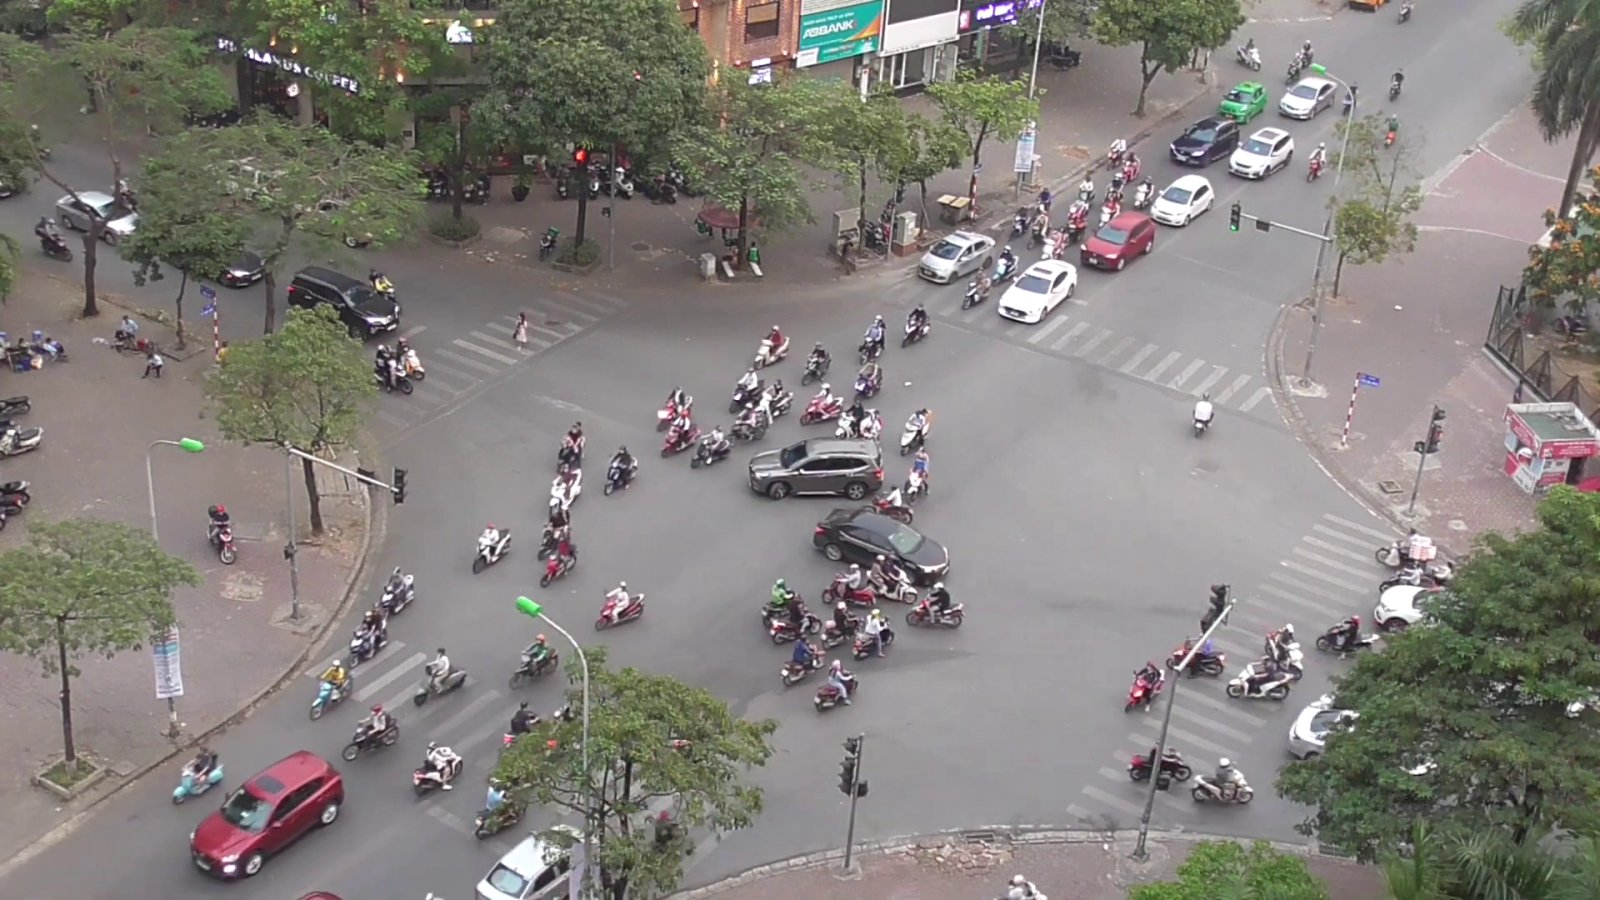
\includegraphics[width=\linewidth]{intro_day.jpg}\caption{Ngã tư ở Hà Nội, ban ngày}\end{subfigure}\hfill
  \begin{subfigure}{0.49\linewidth}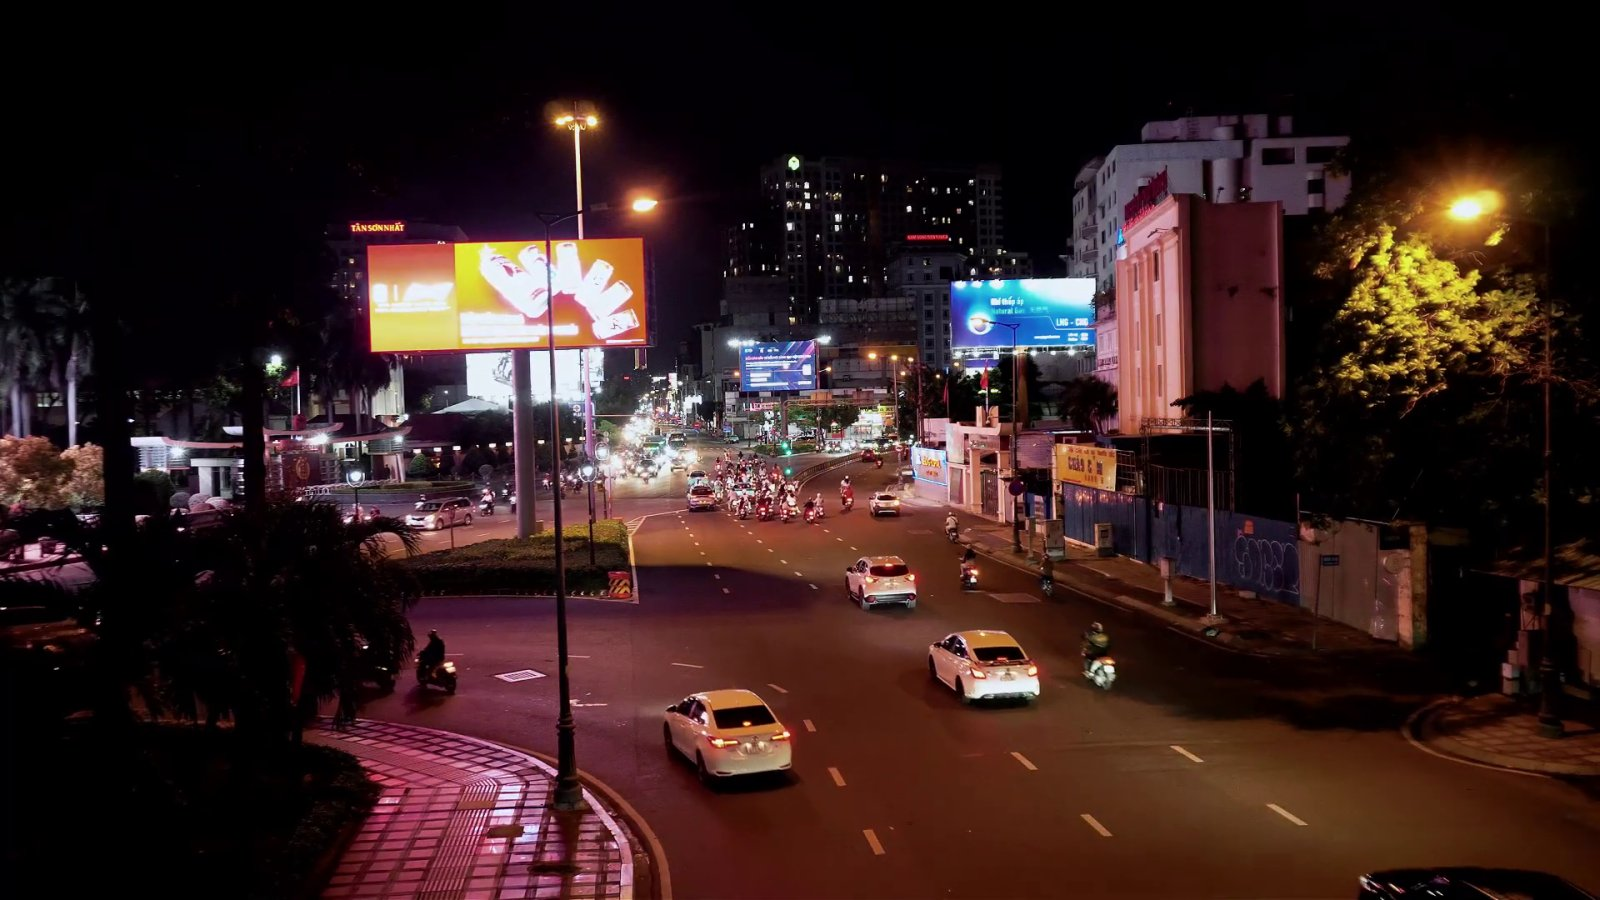
\includegraphics[width=\linewidth]{intro_night.jpg}\caption{Đường phố TP.HCM, ban đêm}\end{subfigure}
  \caption{Giao thông hỗn hợp nhìn từ camera đặt trên cao: xe máy đi dày, xen kẽ ô tô; ban đêm xe chủ yếu hiện ra qua
           đèn xe và đèn đường (nguồn video: kênh YouTube Raw Street Capture 101 và Midnight Soundscape)}
  \label{fig:intro-traffic}
\end{figure}

Hạ tầng để làm việc này bằng camera đang được xây dựng. Tháng 12/2025, Công an thành phố Hà Nội đưa vào vận hành Trung
tâm điều khiển giao thông thông minh, kết nối 1.837 camera tại 195 nút giao; hình ảnh camera được phân tích để xác
định mật độ, lưu lượng phương tiện và điều chỉnh thời gian đèn tín hiệu theo lưu lượng thực tế~\cite{vneconomy2025camera}.
Với số camera lớn như vậy, không thể có người ngồi xem từng màn hình. Để biến video thành số liệu, máy phải tự tìm ra
từng phương tiện trong mỗi frame, cho biết đó là loại xe gì và nhận ra cùng một chiếc xe qua các frame liên tiếp. Đó
chính là ba bài toán phát hiện, phân loại và theo dõi đối tượng.

Các mô hình phát hiện phổ biến thường được huấn luyện sẵn trên bộ dữ liệu COCO, gồm ảnh đời thường chụp ở nhiều nơi
trên thế giới. Cảnh hàng trăm xe máy chở người đi sát nhau, nhìn từ trên cao như ở ngã tư Việt Nam, ít gặp trong bộ dữ
liệu này; COCO còn gán xe máy và người lái thành hai đối tượng riêng. Vì vậy không thể mặc định mô hình huấn luyện sẵn
sẽ chạy tốt trên camera giao thông Việt Nam: cần tinh chỉnh và đo lại trên dữ liệu đúng bối cảnh. Dữ liệu như thế lại
ít. Các bộ dữ liệu xe Việt Nam công khai mà đề tài tìm được phần lớn chỉ gồm một vài camera, góc nhìn chéo từ trên cao
của camera giao thông hầu như không có, và đề tài không tìm được tập cảnh đêm Việt Nam nào có nhãn, trong khi ban đêm
nhiều xe chỉ lộ ra qua đèn pha, đèn hậu (Hình~\ref{fig:intro-traffic}b). Điểm cao trên tập test đi kèm một bộ dữ liệu
cũng chưa đủ để tin mô hình chạy tốt ở camera khác, nên tự xây tập đánh giá đúng bối cảnh là một phần của bài toán.

Về mặt học thuật, đề tài đặt các nội dung chính của môn học vào một bài toán có thật: mạng tích chập và Transformer cho
phát hiện đối tượng, thuật toán theo dõi đa đối tượng, các chỉ số đánh giá chuẩn như mAP và HOTA. Đề tài cũng phải làm
những việc ít gặp khi làm bài tập trên dữ liệu có sẵn: thu thập và gán nhãn dữ liệu, chia tập sao cho con số đo được phản ánh
đúng khả năng tổng quát, cân đối độ chính xác với tốc độ khi máy chỉ là laptop không có GPU rời. Kết quả cuối cùng, số
xe đi qua một vạch, lại dễ kiểm chứng bằng mắt.

Từ những lý do trên, đề tài chọn ứng dụng học sâu vào phát hiện, phân loại và theo dõi phương tiện trong video camera
giao thông Việt Nam, cả ban ngày và ban đêm: tinh chỉnh mô hình phát hiện trên dữ liệu gần bối cảnh mục tiêu, tự xây
các tập đánh giá có người kiểm, rồi kết hợp với thuật toán theo dõi để gán ID cho từng xe và đếm xe qua vạch.

\addsec{Mục tiêu đề tài}

\textbf{Mục tiêu tổng quát:} xây dựng hệ thống phát hiện, phân loại (4 lớp xe máy, ô tô, xe buýt, xe tải) và theo dõi
phương tiện từ video camera giao thông Việt Nam; đánh giá phần phát hiện bằng mAP kiểu COCO và phần theo dõi bằng
HOTA, MOTA, IDF1 theo chuẩn MOTChallenge.

\textbf{Mục tiêu cụ thể:}
\begin{itemize}
  \item Thu thập, gộp và chuẩn hoá dữ liệu huấn luyện từ nhiều nguồn; tự xây các tập test Việt Nam có người kiểm, gồm
        cả cảnh ban đêm, và một clip có nhãn theo dõi.
  \item Tinh chỉnh YOLO26n qua nhiều phiên bản dữ liệu và so sánh với mô hình gốc huấn luyện trên COCO.
  \item So sánh kiến trúc CNN (YOLO26n, YOLO26s) với kiến trúc Transformer (RT-DETRv2-S) theo một giao thức công bằng,
        đo cả độ chính xác lẫn tốc độ.
  \item Chọn và tinh chỉnh thuật toán theo dõi (ByteTrack, BoT-SORT, OC-SORT) trên tập phát triển, rồi chấm cấu hình đã
        chọn trên tập test.
  \item Xây dựng ứng dụng đếm xe qua vạch theo lớp và hướng, đo sai số đếm cả ban ngày và ban đêm; làm web demo bằng
        Streamlit; đo và tối ưu tốc độ trên laptop (CPU, GPU tích hợp, OpenVINO) và trên GPU.
\end{itemize}

\addsec{Giới hạn và phạm vi đề tài}

\textbf{Phạm vi:}
\begin{itemize}
  \item Video từ camera cố định nhìn chéo từ trên cao, kiểu camera giao thông; ban ngày và ban đêm.
  \item Bốn lớp phương tiện: \texttt{motorbike}, \texttt{car}, \texttt{bus}, \texttt{truck}. Box xe máy bao cả người lái.
  \item Góc drone nhìn thẳng xuống và góc ngang tầm mắt chỉ dùng để phân tích lỗi, không tối ưu cho chúng.
\end{itemize}

\textbf{Giới hạn:}
\begin{itemize}
  \item Máy chạy suy luận là laptop không có GPU rời (CPU Intel Core i5-8250U, GPU tích hợp UHD 620); việc huấn luyện
        chạy trên GPU Tesla T4 của Kaggle, với hạn mức khoảng 30 giờ GPU mỗi tuần.
  \item Các tập test do đề tài tự gán nhãn có kích thước nhỏ: 20--30 frame mỗi tập phát hiện, một clip theo dõi dài 20
        giây, và 249 lượt xe qua vạch để đo sai số đếm.
  \item Chỉ v5 và YOLO26s được huấn luyện ba lần với ba seed, mô hình triển khai v6 hai lần; các cấu hình khác mỗi
        cấu hình một lần.
  \item Nhãn của frame huấn luyện (Hà Nội và ban đêm) là nhãn tự động, không có người kiểm từng frame.
\end{itemize}

\addsec{Nội dung thực hiện}

\begin{enumerate}
  \item Dữ liệu: gộp bảy nguồn dữ liệu huấn luyện, chia tập theo cảnh; gán nhãn tay các tập test, một tập dev ban đêm
        và đếm tay số lượt xe qua vạch ở hai clip đêm; tạo nhãn tự động cho frame huấn luyện cắt từ video Hà Nội và
        video đường phố ban đêm.
  \item Huấn luyện: sáu phiên bản YOLO26n (v1 đến v6), một bản YOLO26s và một bản RT-DETRv2-S trên Kaggle;
        v5 và YOLO26s được huấn luyện thêm hai lần, v6 thêm một lần với seed khác.
  \item Theo dõi: so sánh ba thuật toán theo dõi, chỉnh tham số trên tập phát triển VnTraffic, chấm trên clip Phạm Văn
        Đồng gán nhãn tay bằng CVAT.
  \item Ứng dụng: pipeline đếm xe qua vạch, web demo Streamlit, video demo xử lý trên GPU.
  \item Đánh giá qua bốn thí nghiệm: E1 (độ chính xác phát hiện), E2 (tốc độ), E3 (theo dõi và sai số đếm), E4 (phân
        tích lỗi).
\end{enumerate}

\addsec{Phương pháp tiếp cận}

Đề tài kết hợp nghiên cứu tài liệu với thực nghiệm. Phần lý thuyết tổng hợp các mô hình phát hiện họ YOLO và DETR,
các thuật toán theo dõi họ SORT và các chỉ số đánh giá chuẩn. Phần thực nghiệm tuân theo ba nguyên tắc:
\begin{itemize}
  \item Mọi lựa chọn (mô hình, thuật toán theo dõi, kích thước ảnh đầu vào) được quyết định trên tập phát triển (dev)
        theo tiêu chí đặt ra trước khi chạy. Tập test chỉ dùng để báo cáo kết quả, không dùng để chọn; những lần tập
        test được chấm lại được ghi rõ ở mục~\ref{sec:thao-luan}. Hai phương án chênh nhau dưới 0.005 điểm (mAP50 với
        mô hình phát hiện, IDR với theo dõi) được coi là hoà, khi đó chọn phương án nhanh hơn.
  \item Mỗi quyết định đối chiếu với quy ước của các bộ dữ liệu và benchmark lớn (COCO, KITTI, VisDrone, MOTChallenge);
        chỗ nào lệch quy ước thì nêu rõ lý do.
  \item Mọi số liệu trong báo cáo được xuất từ file kết quả của từng lần chạy, kèm cấu hình đã dùng, để có thể truy
        ngược.
\end{itemize}

Báo cáo gồm bốn chương. Chương~\ref{chap:gioithieu} giới thiệu bài toán, ứng dụng và khó khăn.
Chương~\ref{chap:lythuyet} trình bày cơ sở lý thuyết về mô hình phát hiện, thuật toán theo dõi và chỉ số đánh giá.
Chương~\ref{chap:xaydung} mô tả dữ liệu, cách gán nhãn, quá trình huấn luyện và pipeline hệ thống.
Chương~\ref{chap:ketqua} trình bày kết quả thực nghiệm, ứng dụng web, thảo luận, hạn chế và hướng phát triển.
